\documentclass[12pt]{article}  

\usepackage
[colorlinks=true, pdfstartview=FitV, linkcolor=blue, citecolor=blue, urlcolor=blue]
{hyperref}

\usepackage{amssymb}  
\usepackage{amsthm}
\usepackage{amsmath}
\usepackage{graphics} 
\usepackage{graphicx} 
%\usepackage[latin1]{inputenc}
\usepackage{tikz}
\usepackage{pgfplots}
\usepackage{wrapfig}
\usepackage{caption}
\usepgfplotslibrary{polar}
\usepackage{ skull }


% GNUPLOT required
\usepackage{verbatim}

\linespread{1.3}

%\addtolength{\textwidth}{80pt}
\addtolength{\evensidemargin}{20pt}
\addtolength{\oddsidemargin}{20pt}

%%%%%%%%%%%%%%%%%%%%%%%%%%%%%%%%%%%%%%%%%%%%%%
%  Begin user defined commands

\newcommand{\map}[1]{\xrightarrow{#1}}

\newcommand{\N}{\mathbb N}
\newcommand{\Z}{\mathbb Z}
\newcommand{\Primes}{\mathbb P}
\newcommand{\Q}{\mathbb Q}
\newcommand{\R}{\mathbb R}
\newcommand{\C}{\mathbb C}
\newcommand{\bz}{\mathbb Z}
\newcommand{\bq}{\mathbb Q}
\newcommand{\br}{\mathbb R}
\newcommand{\bc}{\mathbb C}
\newcommand{\al}{\alpha}
\newcommand{\be}{\beta}
\newcommand{\ga}{\gamma}
\newcommand{\de}{\delta}
\newcommand{\ep}{\epsilon}
\DeclareMathOperator{\lub}{l.u.b.}
%  End user defined commands
%%%%%%%%%%%%%%%%%%%%%%%%%%%%%%%%%%%%%%%%%%%%%%


%%%%%%%%%%%%%%%%%%%%%%%%%%%%%%%%%%%%%%%%%%%%%%
% These establish different environments for stating Theorems, Lemmas, Remarks, etc.

\newtheorem{Thm}{Theorem}
\newtheorem{Prop}[Thm]{Proposition}
\newtheorem{Lem}[Thm]{Lemma}
\newtheorem{Cor}[Thm]{Corollary}

\theoremstyle{definition}
\newtheorem{Def}[Thm]{Definition}

\theoremstyle{remark}
\newtheorem{Rem}[Thm]{Remark}
\newtheorem{Ex}[Thm]{Example}

\theoremstyle{definition}
\newtheorem{Exercise}{Problem}

\newenvironment{Solution}{\noindent\textbf{Solution.}}{}

%\renewcommand{\labelenumi}{(\alph{enumi})}
\renewcommand\qedsymbol{QED}
% End environments 
%%%%%%%%%%%%%%%%%%%%%%%%%%%%%%%%%%%%%%%%%%%%%%%
%Some commands to save paper


\setlength{\parindent}{0in}
\setlength{\parskip}{8pt}

\DeclareMathOperator{\arcsec}{arcsec}
\DeclareMathOperator{\arccot}{arccot}
\DeclareMathOperator{\arccsc}{arccsc}
\DeclareMathOperator{\LH}{\ \underset{\text{LH}}{=}\ }
\newcommand{\Dep}{\Delta_+}
\newcommand{\Dem}{\Delta_-}
\newcommand{\bu}{\mathbf u}
\newcommand{\bv}{\mathbf v}
\newcommand{\bw}{\mathbf w}

\newcommand{\ora}{\overrightarrow}



\addtolength{\textwidth}{80pt}
\addtolength{\evensidemargin}{-40pt}
\addtolength{\oddsidemargin}{-40pt}
\addtolength{\topmargin}{-80pt}
\addtolength{\textheight}{1.8in}

\setlength{\parindent}{0in}
\setlength{\parskip}{8pt}

\DeclareMathOperator{\arcsinh}{arcsinh}

%%%%%%%%%%%%%%%%%%%%%%%%%%%%%%%%%%%%%%%%%%%%%%
% Now we're ready to start
%%%%%%%%%%%%%%%%%%%%%%%%%%%%%%%%%%%%%%%%%%%%%%

\begin{document}  

%\author{Your Name}
{\bf MATH 1103 Homework 3}\\
{\bf Due Friday February 9, 2018}


Practice Problems (not to be turned in)



{\bf Practice 1.\ }  Consider the two sequences 
\[x_1=-\frac{2}{3},\quad x_2=-\frac{4}{9}, \quad x_3=-\frac{8}{27},\dots\qquad\text{and}\qquad y_1=\frac{2}{3},\quad y_2=\frac{4}{9}, \quad y_3=\frac{8}{27},\dots\]
a)\ Find a formula for $x_n$ and $y_n$ for general $n$. 

b)\ Show that $x_n$ and $y_n$ satisfy the conditions of the Zax theorem and find the number $z$ in that theorem. 

{\bf Practice 2.\ }  Find two sequences $(x_n)$ and $(y_n)$ such that $(x_n-y_n)$ is monotone decreasing, with limit equal to zero, but the sequences $(x_n)$ and $(y_n)$ themselves diverge. 


\vskip5pt
{\bf Practice 3.\ } Determine whether the following series converge or diverge, and find the sum of those that converge.

a)\ 
\[\frac{1}{10000}+\frac{1}{10001}+\frac{1}{10002}+\frac{1}{10003}+\cdots\]

%Diverges. This is the Harmonic series, after finitely many terms. 

b)\ 
\[\frac{1}{10000}+\frac{1}{20000}+\frac{1}{30000}+\frac{1}{40000}+\cdots\]

%Diverges. This is $1/10000$ times the Harmonic series.

c)\
\[\frac{1}{10000}+\frac{1}{20000}+\frac{1}{40000}+\frac{1}{80000}+\cdots\]

%Converges. This is $1/10000$ times the geometric series $1+\frac{1}{2}+\frac{1}{4}+\cdots$, so it converges, and the sum is
%\[\frac{1}{10000}\left(1+\frac{1}{2}+\frac{1}{4}+\dots\right)=
%\frac{1}{10000}\cdot 2=\frac{1}{5000}.
%\]





{\bf Practice 4.\ }   Show that the following series converges and find the sum.

\[\!\quad\qquad\qquad 1+\frac{1}{2}+\frac{1}{3}+\frac{1}{4}+\frac{1}{6}+\frac{1}{8}+\frac{1}{9}+\frac{1}{12}+\frac{1}{16}+\frac{1}{18}+\cdots
\]
Hint: Consider the series $(1+\frac{1}{2}+\frac{1}{4}+\frac{1}{8}+\dots)$ and $(1+\frac{1}{3}+\frac{1}{9}+\frac{1}{27}+\dots)$.

%\begin{Solution} 
%The series in question is the product of the two series in the hint, which are geometric series with sums $2$ and $3/2$, respectively, 
%so 
%\[1+\frac{1}{2}+\frac{1}{3}+\frac{1}{4}+\frac{1}{6}+\frac{1}{8}+\frac{1}{9}+\frac{1}{12}+\frac{1}{16}+\frac{1}{18}+\cdots=2\cdot\frac{3}{2}=3.
%\end{Solution}

{\bf Practice 5.\ } a) Find the sum of the  series
$\sum\limits_{n=1}^\infty\dfrac{1}{n(n+3)}$. 
Hint:$ \dfrac{1}{n(n+3)}=\dfrac{1}{3}\left[\dfrac{1}{n}-\dfrac{1}{n+3}\right]$.
Use the same method to express the sum 
\[\sum_{n=1}^\infty\frac{1}{n(n+k)}\]
in terms of the Harmonic Number $H_k=1+\frac{1}{2}+\frac{1}{3}+\frac{1}{4}+\cdots+\frac{1}{k}$. 

%\begin{Solution} \end{Solution}

 \rule{\textwidth}{1pt}
The homework to be turned in may be found on the next page.


\newpage

{\bf Homework 3 problems to be turned in.}

{\bf 1.\ } Use the Zax Theorem to prove that the sequence $(z_n)$ given by 
\[z_n=\frac{1}{2}-\frac{1}{3}+\frac{1}{5}-\cdots+\frac{(-1)^n}{n}
\] 
converges. (You don't have to find the limit.) 
%\begin{Solution} \end{Solution}

{\bf 2.\ }  The  {\bf geometric mean} of two numbers $0\leq a\leq b$ is $\sqrt{ab}$. Their {\bf arithmetic mean} is $(a+b)/2$.
Prove that the sequences $(a_n)$ and $(b_n)$ defined by $a_0=a,\ b_0=b$, 
\[a_{n+1}=\sqrt{a_nb_n},\qquad b_{n+1}=\frac{a_n+b_n}{2}\]
are Zax, and that $b_n-a_n\to 0$. 

{\bf comment:\ } According to the Zax theorem there is a unique number $M(a,b)$ such that $a_n\leq M(a,b)\leq b_n$ for all $n$. This is the {\bf arithmetic-geometric mean} of $a,b$, otherwise known as the AGM. Application: The period $T$ of a simple pendulum of length $L$  with maximum angle $\al$ is given by 
\[T=\frac{2\pi\sqrt{L/g}}{M(\cos(\al/2),1)}.
\]


The next two problems follow section 3.1 of the notes. 

{\bf 3.\ } Prove that $\sqrt{5}$ is irrational.

%\begin{Solution} \end{Solution}

\vskip10pt

{\bf 4.\ } Let
\[z=
1+\cfrac {1}{1+ \cfrac{ 1}{1+ \cfrac{ 1}{1+ \cfrac{ 1}{1+ \ddots}}}} .
\]

a)\ Find a quadratic equation for $z$ by locating $z$ inside of itself, and use this equation to find $z$.

b)\  Consider the sequence $(z_n)$ given recursively by $z_0=1$, $z_{n+1}=1+\dfrac{1}{z_n}$. 
Let $x_n=z_{2n}$ and $y_n=z_{2n+1}$. Compute $x_n, y_n$ for $n=0,1,2,3$, and show that for these $n$, the sequences $(x_n)$ and $(y_n)$ satisfy the Zax conditions. 

c)\ Compute $y_n-x_n$ for $n=0,1,2,3$ and make a conjecture about $y_n-x_n$ for any positive integer $n$. You do not have to prove your conjecture.

d)\ Assume that your conjecture in c) is correct. Prove that $z$ above is the unique number larger than all $x_n$ and smaller than all $y_n$, as in the Zax Theorem.

e)\ Look up ``Fibonacci" on the interwebs (not graded!) 

%\begin{Solution} \end{Solution} 


{\bf 5.\ } The goal of this exercise is to sum the series $r+2r^2+3r^3+\cdots$ when $0<r<1$. 

a)\ Differentiate, with respect to $r$, both sides of the Geometric Expansion
\[1+r+r^2+\cdots+r^{n}=\frac{1-r^{n+1}}{1-r},\]
being sure to simplify the right-hand side. 

%Differentiating both sides and simplifying gives
%\[
%1+2x+3x^2+4x^3+\cdots+nx^{n-1}=\frac{nx^{n+1}-(n+1)x^n+1}{(1-x)^2}.
%\]

b)\ Use your result in a) and some algebra to find an identity for 
\[r+2r^2+3r^3+\cdots +n r^n\]
which is similar to the Geometric Expansion. 
%We have
%\[x+2x^2+3x^3+\cdots +n x^n
%=x\cdot\left(1+2x+3x^2+4x^3+\cdots+nx^{n-1}\right)
%=x\cdot\frac{nx^{n+1}-(n+1)x^n+1}{(1-x)^2}.
%\]


c)\ Use your result in b) to show that the series \[\sum_{k=1}^\infty k r^k\]
converges if $0<r<1$ and find the sum in that case. 

%If $0<r<1$ we have $n x^n\to 0$ as $n\to\infty$, so 
%\[\sum_{k=1}^\infty k x^k=
%\lim_{n\to\infty}
%x\cdot\frac{nx^{n+1}-(n+1)x^n+1}{(1-x)^2}=\frac{x}{(1-x)^2}.
%\]


 
{\bf 6.\ } The picture below shows the graphs of $y=x^n$ for $n=0,1,2,3,4\dots$ dividing the square $0\leq x,y\leq 1$ into infinitely many zones. 

a)\ Use Fermat's quadrature of $y=x^n$ to find the area of each zone. 

b)\ Use your answer to a) to find the sum of the infinite series
$\sum\limits_{n=1}^\infty\dfrac{1}{n(n+1)}$. 

\begin{center}
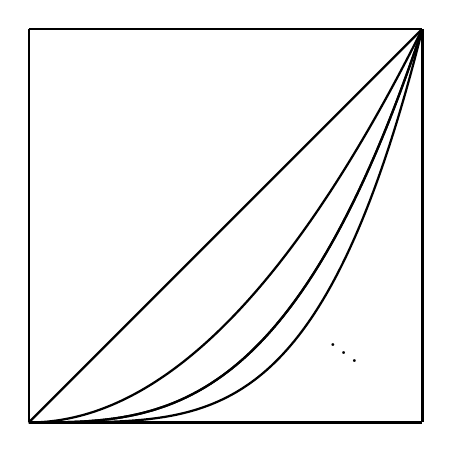
\begin{tikzpicture}[samples=100, domain=0:1, scale=5]
\draw[black,   thick] (0,0) -- (1,0 );
\draw[black,   thick] (0,0) -- (0,1 );
\draw[black,   thick] (1,0) -- (1,1);
\draw[black,   thick] (0,1) -- (1,1 );
%\node[label=below: $0$] at (0,0) {};
%\node[label=below: $1$] at (1,0) {};
\node[label=below: ${\ddots}$] at (.8, .3) {};
\draw[black, thick] plot [domain=0: 1 ] (\x,{\x)}) ;
\draw[black, thick] plot [domain=0: 1 ] (\x,{\x*\x)}) ;
\draw[black, thick] plot [domain=0: 1 ] (\x,{\x*\x*\x)}) ;
\draw[black, thick] plot [domain=0: 1 ] (\x,{\x*\x*\x)}) ;
\draw[black, thick] plot [domain=0: 1 ] (\x,{\x*\x*\x*\x)}) ;
%\fill[fill=cyan!40!](0,0) -- plot [domain=0:4, ] (\x,{(1/4)*\x*\x)}) -- (4,0) -- cycle;
%\draw [black,  thick] (4,0) -- (4,.64*4);
\end{tikzpicture}
\end{center}

\begin{Solution} 
\end{Solution}









\end{document}

 
 
